%%%%%%%%%%%%%%%%%%%%%%%%%%%%%%%%%%%%%%%%%
% Jacobs Landscape Poster
% LaTeX Template
% Version 1.1 (14/06/14)
%
% Created by:
% Computational Physics and Biophysics Group, Jacobs University
% https://teamwork.jacobs-university.de:8443/confluence/display/CoPandBiG/LaTeX+Poster
% 
% Further modified by:
% Nathaniel Johnston (nathaniel@njohnston.ca)
%
% This template has been downloaded from:
% http://www.LaTeXTemplates.com
%
% License:
% CC BY-NC-SA 3.0 (http://creativecommons.org/licenses/by-nc-sa/3.0/)
%
%%%%%%%%%%%%%%%%%%%%%%%%%%%%%%%%%%%%%%%%%

% This template has been modified by:
%       Jonathan Sumner Evans (jonathanevans@mines.edu)
%       Sam Sartor (ssartor@mines.edu)
%       Robbie Merillat (rdmerillat@mines.edu)


%----------------------------------------------------------------------------------------
%	PACKAGES AND OTHER DOCUMENT CONFIGURATIONS
%----------------------------------------------------------------------------------------

\documentclass[final]{beamer}

\usepackage[scale=1.3]{beamerposter} % Use the beamerposter package for laying out the poster
\usepackage{biblatex}
\usepackage{csquotes}
\usepackage{enumitem}
\usepackage{graphicx}
\usepackage{subcaption}
\usepackage{booktabs} % Top and bottom rules for tables

\usetheme{confposter} % Use the confposter theme supplied with this template

\addbibresource{../report/references.bib}

\setbeamercolor{block title}{fg=ngreen,bg=white} % Colors of the block titles
\setbeamercolor{block body}{fg=black,bg=white} % Colors of the body of blocks
\setbeamercolor{block alerted title}{fg=white,bg=dblue!70} % Colors of the highlighted block titles
\setbeamercolor{block alerted body}{fg=black,bg=dblue!10} % Colors of the body of highlighted blocks
% Many more colors are available for use in beamerthemeconfposter.sty

%-----------------------------------------------------------
% Define the column widths and overall poster size
% To set effective sepwid, onecolwid and twocolwid values, first choose how many columns you want and how much separation you want between columns
% In this template, the separation width chosen is 0.024 of the paper width and a 4-column layout
% onecolwid should therefore be (1-(# of columns+1)*sepwid)/# of columns e.g. (1-(4+1)*0.024)/4 = 0.22
% Set twocolwid to be (2*onecolwid)+sepwid = 0.464

\newlength{\sepwid}
\newlength{\onecolwid}
\newlength{\twocolwid}
\setlength{\paperwidth}{48in} % A0 width: 46.8in
\setlength{\paperheight}{36in} % A0 height: 33.1in
\setlength{\sepwid}{0.024\paperwidth} % Separation width (white space) between columns
\setlength{\onecolwid}{0.3\paperwidth} % Width of one column
\setlength{\twocolwid}{0.6\paperwidth} % Width of two columns
\setlength{\topmargin}{-0.5in} % Reduce the top margin size

%-----------------------------------------------------------

\title{Exploration of Virtual Reality and Deferred Immediate Mode}
\author{Jonathan Sumner Evans, Robinson Merillat, and Sam Sartor}
\institute{Department of Computer Science, Colorado School of Mines}

\begin{document}

    \addtobeamertemplate{block end}{}{\vspace*{2ex}} % White space under blocks
    \addtobeamertemplate{block alerted end}{}{\vspace*{2ex}} % White space under highlighted (alert) blocks

    \setlength{\belowcaptionskip}{2ex} % White space under figures
    \setlength\belowdisplayshortskip{2ex} % White space under equations

    \begin{frame}[t] % The whole poster is enclosed in one beamer frame
        % The whole poster consists of three major columns, the second of which
        % is split into two columns twice - the [t] option aligns each column's
        % content to the top
        \begin{columns}[t]
            \begin{column}{\sepwid}\end{column} % Empty spacer column

            \begin{column}{\onecolwid} % The first column

                \begin{block}{Goals}

                    We set out to find a system that provides a modern, fast,
                    and practical approach to virtual reality development.
                    Specifically, we needed a framework which met the
                    following criteria:

                    \begin{enumerate}[leftmargin=8.75cm, labelsep=1cm]

                        \item[\textbf{Performant}] VR requires at least 90
                            frames per second to run smoothly. Low frame rates
                            can cause users to experience headaches and nausea
                            faster than when at high frame rates~\cite{irisVR}.
                            This requires VR programs to be highly optimized and
                            multi-threadable.

                        \item[\textbf{Natural}] VR enables new user interfaces
                            where components are organized within a 3D space. We
                            wanted such components to be first class.

                        \item[\textbf{Flexible}] We need a general purpose user
                            interface toolkit designed specifically for VR.

                        \item[\textbf{Modular}] We need a toolkit which does
                            not include unnecessary features, but is extensible
                            with modular components.

                    \end{enumerate}

                \end{block}

                \begin{block}{Exploration}

                    Over the course of many months, we explored several existing
                    VR frameworks and application architectures. We determined
                    that none of them meet our criteria for VR development.

                    We created our own user interface and rendering framework
                    which addresses the problems that we encountered during our
                    exploration. We initially made use of the immediate mode
                    program architecture because of its flexibility and
                    extensibility, but repeatedly ran into the following
                    problem:

                    \begin{quote}

                        \textbf{There are some questions about the state of the
                        system which cannot be answered until all system
                        elements have ``reported'' their state.}

                    \end{quote}

                    To solve this problem, we created a powerful new program
                    architecture called \textbf{Deferred Immediate Mode (DIM)}.
                    The addition of \textit{deferrability} to the classic
                    immediate mode architecture solves our issues with
                    interdependent user interface elements without sacrificing
                    flexibility.

                    The DIM architecture enabled us to meet all of our goals for
                    effective VR application development.

                \end{block}

            \end{column} % End of the first column

            \begin{column}{\sepwid}\end{column} % Empty spacer column

            \begin{column}{\onecolwid} % Start of column 2

                \begin{block}{Flight}
                    \setlength{\parskip}{0.5em}

                    Our virtual reality toolkit, called flight, features high
                    level abstractions for interacting with VR hardware, a
                    state-of-the-art real-time rendering engine, asset loading
                    tools, and a selection of built-in UI elements. Flight is
                    designed from the ground up to be performant, general, and
                    modular.

                \end{block}

                \begin{figure}[H]
                    \centering
                    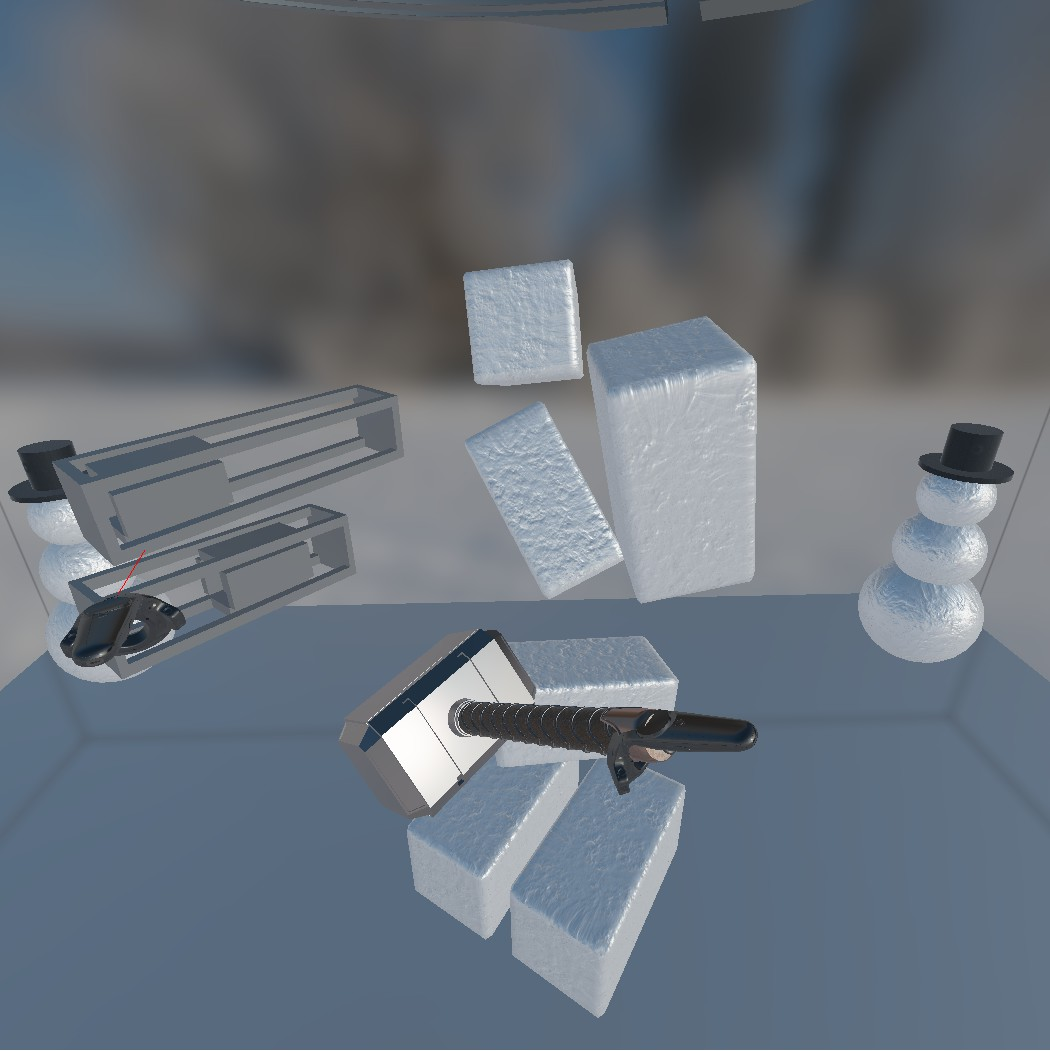
\includegraphics[width=0.9\linewidth]{../report/screenshots/physics_b.jpg}
                    \caption{Our Final Project}\label{fig:project}
                \end{figure}

                \begin{block}{References}
                    \printbibliography
                \end{block}

                \setbeamercolor{block alerted title}{fg=black,bg=norange} % Change the alert block title colors
                \setbeamercolor{block alerted body}{fg=black,bg=white} % Change the alert block body colors

                \begin{alertblock}{More Information}

                    \begin{enumerate}[leftmargin=6.5cm, labelsep=1cm]

                        \item[\textbf{Project}]
                            \href{https://github.com/CSM-Dream-Team/final-project}{\url{github.com/CSM-Dream-Team/final-project}}

                        \item[\textbf{Flight}]
                            \href{https://github.com/flight-rs/flight}{\url{github.com/flight-rs/flight}}
                    \end{enumerate}

                \end{alertblock}
            \end{column} % End of column 2

            \begin{column}{\sepwid}\end{column} % Empty spacer column

            \begin{column}{\onecolwid} % Start of third column

                \begin{block}{Final Project}
                    \setlength{\parskip}{0.5em}

                    Our final project demonstrates the results of using DIM to
                    implement a complex VR application. The environment
                    currently provides these features:
                    \begin{itemize}

                        \item \textbf{Modularity:} Each part of the application
                            is its own isolated module that can be modified and
                            even turned off without interfering with other
                            modules.
                            \begin{figure}[H]
                                \begin{subfigure}{0.5\linewidth}
                                    \centering
                                    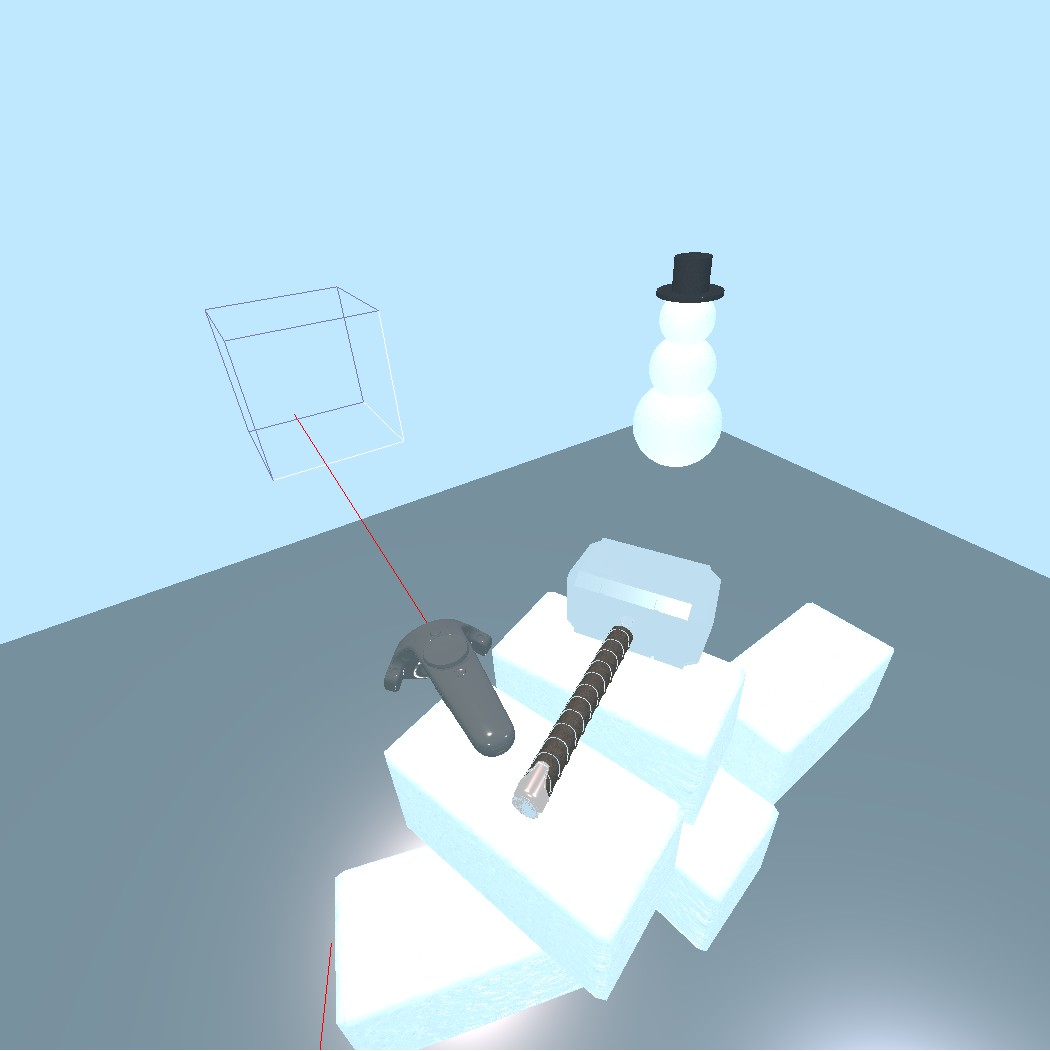
\includegraphics[width=0.95\linewidth]{../report/screenshots/toggle_a.jpg}
                                    \caption{Before}
                                \end{subfigure}%
                                \begin{subfigure}{0.5\linewidth}
                                    \centering
                                    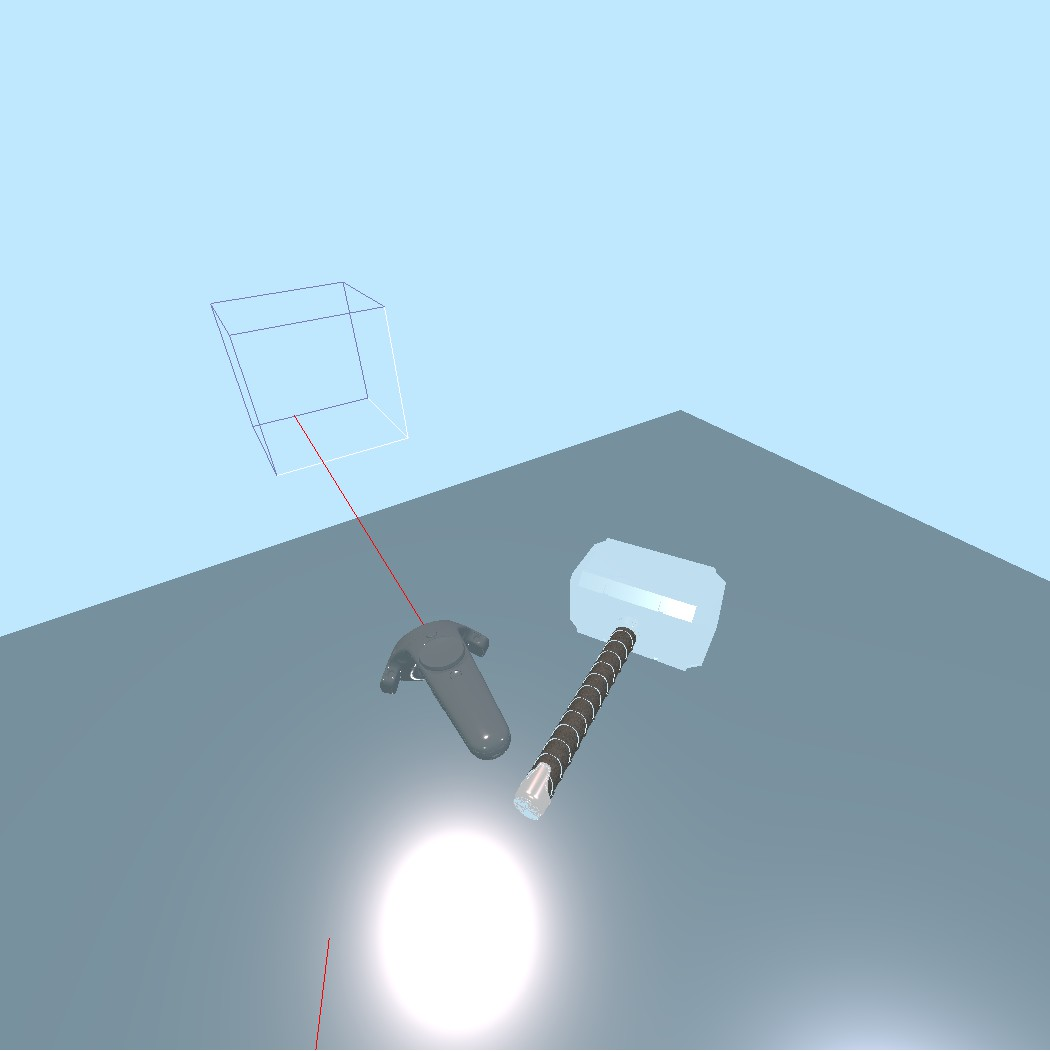
\includegraphics[width=0.95\linewidth]{../report/screenshots/toggle_b.jpg}
                                    \caption{After}
                                \end{subfigure}
                                \caption{Application Toggles}\label{fig:toggles}
                            \end{figure}

                        \item \textbf{Inter-Application Physics:} Althogh each
                            application is in a seprate module, DIM allows them
                            to interact seemlessly. For example, Mjolnir can hit
                            snowblocks.

                        \item \textbf{Yanking, Grabbing, and Pointing:} All
                            elements which can be grabbed, yanked, or pointed at
                            are manipulated using a common, intuitive user
                            interface scheme.

                            \begin{figure}[H]
                                \centering
                                \begin{subfigure}{0.5\linewidth}
                                    \centering
                                    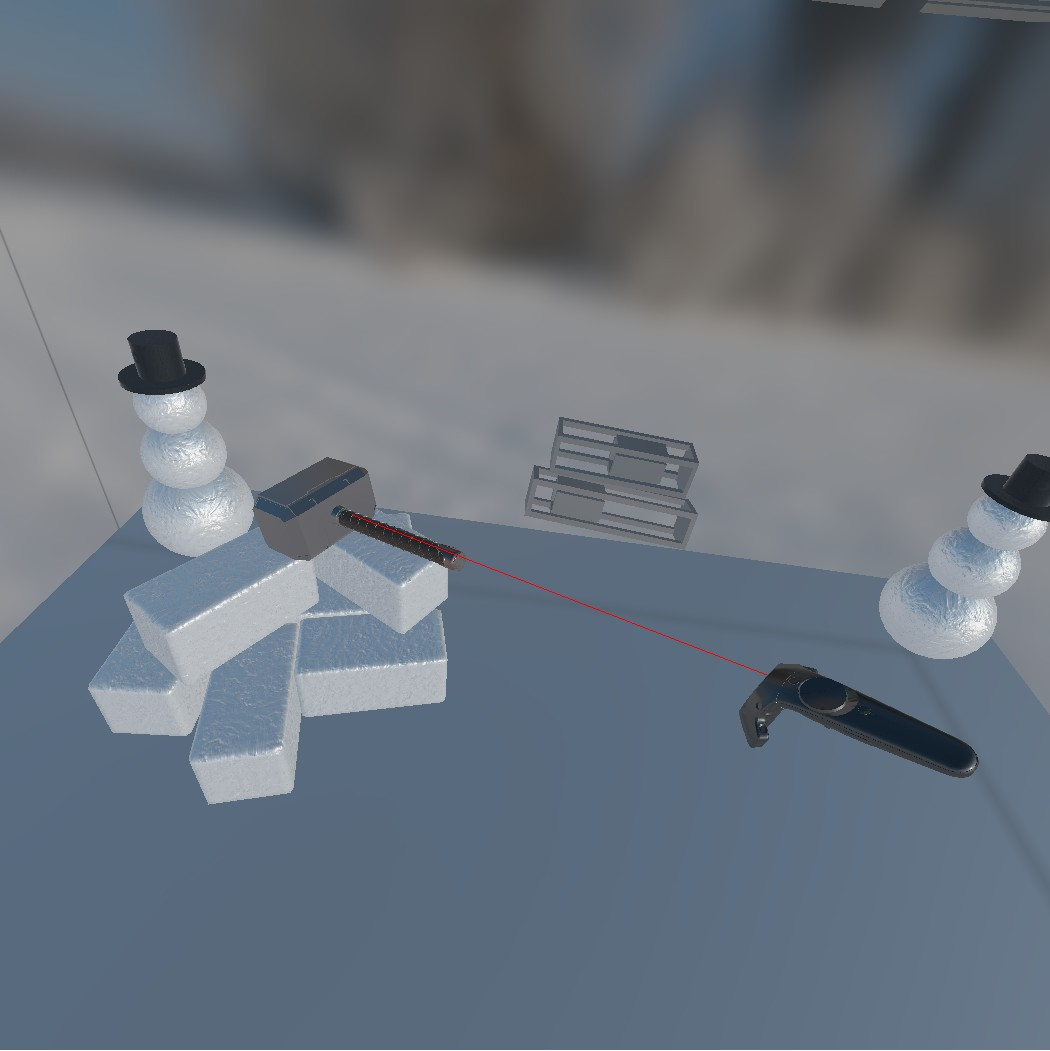
\includegraphics[width=0.95\linewidth]{../report/screenshots/yank_a.jpg}
                                    \caption{Before}
                                \end{subfigure}%
                                \begin{subfigure}{0.5\linewidth}
                                    \centering
                                    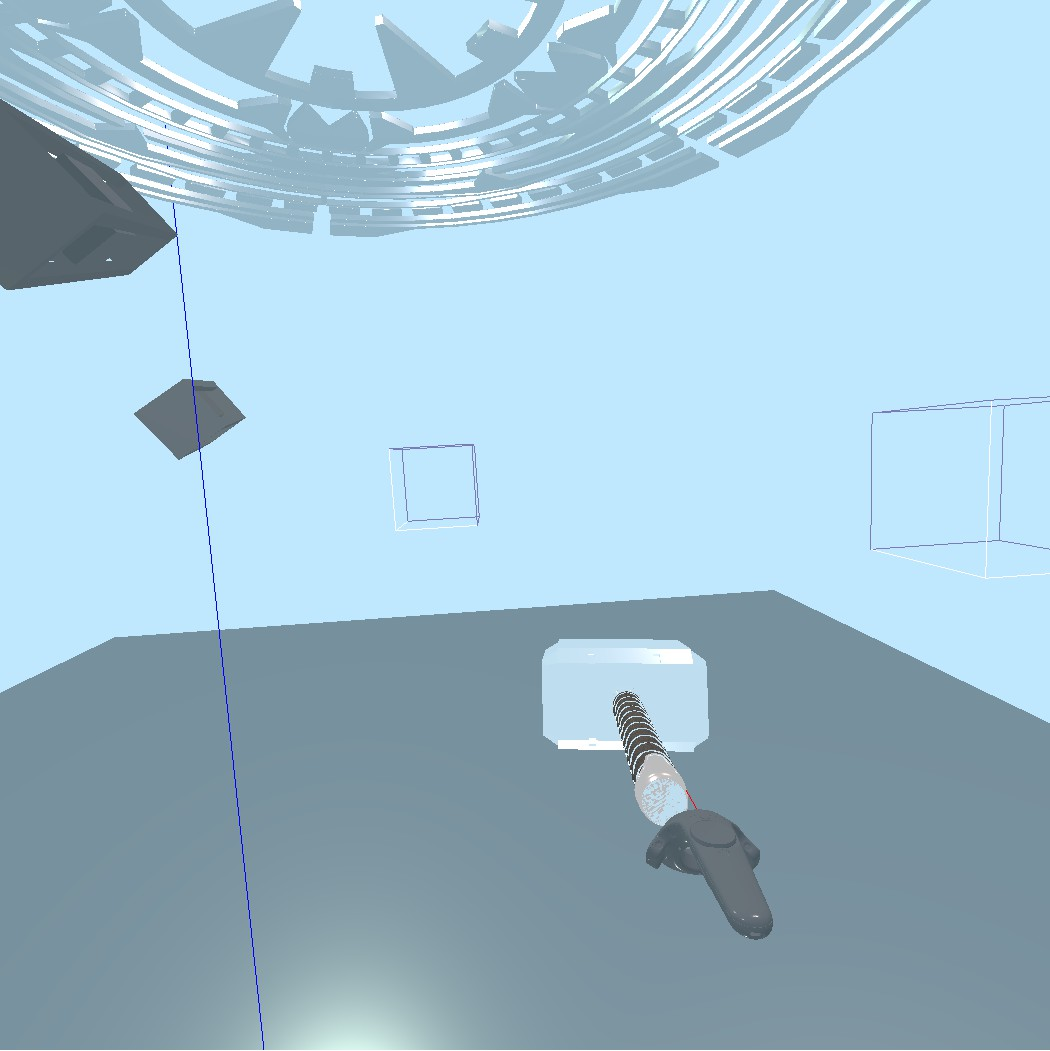
\includegraphics[width=0.95\linewidth]{../report/screenshots/yank_b.jpg}
                                    \caption{After}
                                \end{subfigure}
                                \caption{Yanking Mjolnir from a Distance}\label{fig:physics}
                            \end{figure}
                    \end{itemize}

                \end{block}

            \end{column} % End of the third column

        \end{columns} % End of all the columns in the poster

    \end{frame} % End of the enclosing frame

\end{document}
